\documentclass[11pt]{article}
\usepackage{amsmath, amssymb, amsthm}
\usepackage[retainorgcmds]{IEEEtrantools}

\usepackage[pdftex]{graphicx}

\usepackage{fancyhdr}

%Listings stuff
\usepackage{listings}
\usepackage{lstautogobble}
\usepackage{color}

\definecolor{gray}{rgb}{0.5,0.5,0.5}
\lstset{
basicstyle={\small\ttfamily},
tabsize=3,
numbers=left,
numbersep=5pt,
numberstyle=\tiny\color{gray},
stepnumber=2,
breaklines=true
}

%Format stuff
\pagestyle{fancy}
\headheight 35pt

%Header info
\chead{\Large \textbf{Course Introduction}}
\lhead{}
\rhead{}

\begin{document}
\section{Introduction to C}
	C compiles to machine code, not bytecode like Java. There is no explicit support for object-oriented programming. Array bounds, memory leaks, and errors are all up to the programmer to handle.

	\begin{lstlisting}[autogobble=true]
		#include<stdio.h>
		
		int main() {
			printf("Hello World!\n");
			return 0;
		}
	\end{lstlisting}
	
\section{Instruction-Based Execution}
	Assembly language is processor-specific and is about as close to true machine code as programmers want to deal with. Example of an arbitrary assembly language:

	\begin{lstlisting}[autogobble=true]
		main:	mov	#0,sum			;	set sum to 0
				mov	#1,num			;	set num to 1
		loop:	add	num,sum			;	add num to sum
				add	#1,num			;	add 1 to num
				ble	num,#1000,loop	;	if num <=1000, goto loop
				halt				;	end	
	\end{lstlisting}
	
	Note that the sequence of operations doesn't always go to the next instruction in memory - there is not an explicit linear flow.
	
\section{Computer Layout}
	Memory heirarchy:
	\begin{itemize}
		\item CPU registers
		\item CPU caches
		\item Main memory (RAM)
		\item Hard drives
		\item Remote storage
	\end{itemize}
	
	Generally, the farther away from the CPU, the longer it takes to access data (Figure \ref{fig:memory}).
	
	\begin{figure}[htb]
		\centering
		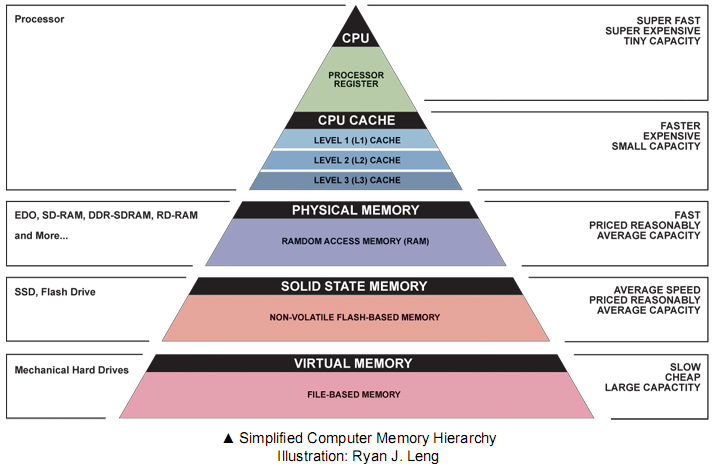
\includegraphics[width=0.8\textwidth]{hei.png}
		\caption{Simplified memory heirarchy diagram}
		\label{fig:memory}
	\end{figure}
	
	Because of the costs involved with accessing data, caching is important. A program can create local copies of blocks of data in main memory or caches to speed up access.

\section{Operating System}
	The primary roles of the operating system are to protect the computer from misuse and abstract the hardware. The OS manages resources to allow for use by all users and programs.
		
\section{Processes}
	Programs are written as if they are the only things running on a system. A process is a running instance of a program along with all data associated with it, and is an abstraction provided by the OS. The OS will switch between different \textbf{contexts} to give the appearance of multiple processes executing at once on a single processor.
	
	\subsection{Virtual Memory}
		Each process is given the appearance of having 4GB of available memory (on a 32-bit system) - this is virtual memory. Virtual memory is not equivalent to actual, physical memory, and the addresses in virtual memory are mapped to actual memory addresses in a \textbf{page table}.
		
		Memory is organized from top to bottom in terms of addresses, with program code and data on the bottom, heap above, and the stack on top. The stack grows downwards while the heap grows upwards.
		
	\begin{figure}[htb]
		\centering
		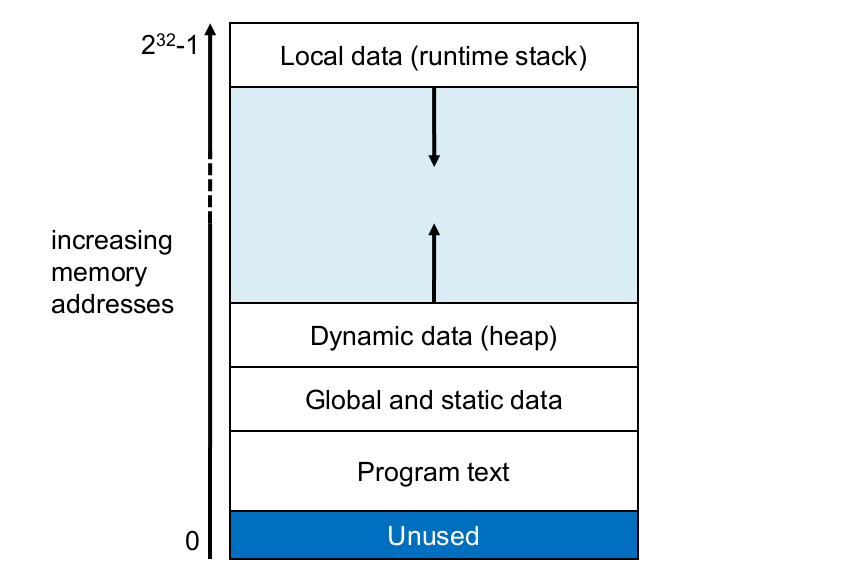
\includegraphics[width=0.8\textwidth]{vmem.png}
		\caption{Simplified diagram of segmented virtual memory for a C program.}
		\label{fig:virtual memory}
	\end{figure}
	
\section{Files in UNIX}
	In UNIX, all I/O devices are modeled as a file, a sequence of bytes in memory - not a container or any other abstraction, just the bytes. All devices are treated as if they are files in UNIX, so they are accessed the same way.

%	\begin{center}
%	\begin{tikzpicture}
%		[scale=3,line cap=round,
%		%Styles
%		axes/.style=,
%		important line/.style={very thick},
%		information text/.style={rounded corners,fill=red!10,inner sep=1ex},
%		dot/.style={circle,inner sep=1pt,fill,label={#1},name=#1}			
%		]
%		
%		%Colors
%		\colorlet{anglecolor}{green!50!black}	%angle arcs/lines
%		
%		%The graphic
%	\end{tikzpicture}
%	\end{center}

%	\begin{figure}[htb]
%		\centering
%		\includegraphics[width=0.8\textwidth]{filename.eps}
%		\caption{Caption.}
%		\label{fig:figure}
%	\end{figure}

%		\def\enotesize{\normalsize}
%		\theendnotes
\end{document}